% Options for packages loaded elsewhere
\PassOptionsToPackage{unicode}{hyperref}
\PassOptionsToPackage{hyphens}{url}
%
\documentclass[
]{article}
\usepackage{amsmath,amssymb}
\usepackage{lmodern}
\usepackage{ifxetex,ifluatex}
\ifnum 0\ifxetex 1\fi\ifluatex 1\fi=0 % if pdftex
  \usepackage[T1]{fontenc}
  \usepackage[utf8]{inputenc}
  \usepackage{textcomp} % provide euro and other symbols
\else % if luatex or xetex
  \usepackage{unicode-math}
  \defaultfontfeatures{Scale=MatchLowercase}
  \defaultfontfeatures[\rmfamily]{Ligatures=TeX,Scale=1}
\fi
% Use upquote if available, for straight quotes in verbatim environments
\IfFileExists{upquote.sty}{\usepackage{upquote}}{}
\IfFileExists{microtype.sty}{% use microtype if available
  \usepackage[]{microtype}
  \UseMicrotypeSet[protrusion]{basicmath} % disable protrusion for tt fonts
}{}
\makeatletter
\@ifundefined{KOMAClassName}{% if non-KOMA class
  \IfFileExists{parskip.sty}{%
    \usepackage{parskip}
  }{% else
    \setlength{\parindent}{0pt}
    \setlength{\parskip}{6pt plus 2pt minus 1pt}}
}{% if KOMA class
  \KOMAoptions{parskip=half}}
\makeatother
\usepackage{xcolor}
\IfFileExists{xurl.sty}{\usepackage{xurl}}{} % add URL line breaks if available
\IfFileExists{bookmark.sty}{\usepackage{bookmark}}{\usepackage{hyperref}}
\hypersetup{
  pdftitle={Can R Notebooks help with reproducibility?},
  pdfauthor={Av Ann Elisabeth Jacobsen og Heidi Marie Rolfsnes},
  hidelinks,
  pdfcreator={LaTeX via pandoc}}
\urlstyle{same} % disable monospaced font for URLs
\usepackage[margin=1in]{geometry}
\usepackage{color}
\usepackage{fancyvrb}
\newcommand{\VerbBar}{|}
\newcommand{\VERB}{\Verb[commandchars=\\\{\}]}
\DefineVerbatimEnvironment{Highlighting}{Verbatim}{commandchars=\\\{\}}
% Add ',fontsize=\small' for more characters per line
\usepackage{framed}
\definecolor{shadecolor}{RGB}{248,248,248}
\newenvironment{Shaded}{\begin{snugshade}}{\end{snugshade}}
\newcommand{\AlertTok}[1]{\textcolor[rgb]{0.94,0.16,0.16}{#1}}
\newcommand{\AnnotationTok}[1]{\textcolor[rgb]{0.56,0.35,0.01}{\textbf{\textit{#1}}}}
\newcommand{\AttributeTok}[1]{\textcolor[rgb]{0.77,0.63,0.00}{#1}}
\newcommand{\BaseNTok}[1]{\textcolor[rgb]{0.00,0.00,0.81}{#1}}
\newcommand{\BuiltInTok}[1]{#1}
\newcommand{\CharTok}[1]{\textcolor[rgb]{0.31,0.60,0.02}{#1}}
\newcommand{\CommentTok}[1]{\textcolor[rgb]{0.56,0.35,0.01}{\textit{#1}}}
\newcommand{\CommentVarTok}[1]{\textcolor[rgb]{0.56,0.35,0.01}{\textbf{\textit{#1}}}}
\newcommand{\ConstantTok}[1]{\textcolor[rgb]{0.00,0.00,0.00}{#1}}
\newcommand{\ControlFlowTok}[1]{\textcolor[rgb]{0.13,0.29,0.53}{\textbf{#1}}}
\newcommand{\DataTypeTok}[1]{\textcolor[rgb]{0.13,0.29,0.53}{#1}}
\newcommand{\DecValTok}[1]{\textcolor[rgb]{0.00,0.00,0.81}{#1}}
\newcommand{\DocumentationTok}[1]{\textcolor[rgb]{0.56,0.35,0.01}{\textbf{\textit{#1}}}}
\newcommand{\ErrorTok}[1]{\textcolor[rgb]{0.64,0.00,0.00}{\textbf{#1}}}
\newcommand{\ExtensionTok}[1]{#1}
\newcommand{\FloatTok}[1]{\textcolor[rgb]{0.00,0.00,0.81}{#1}}
\newcommand{\FunctionTok}[1]{\textcolor[rgb]{0.00,0.00,0.00}{#1}}
\newcommand{\ImportTok}[1]{#1}
\newcommand{\InformationTok}[1]{\textcolor[rgb]{0.56,0.35,0.01}{\textbf{\textit{#1}}}}
\newcommand{\KeywordTok}[1]{\textcolor[rgb]{0.13,0.29,0.53}{\textbf{#1}}}
\newcommand{\NormalTok}[1]{#1}
\newcommand{\OperatorTok}[1]{\textcolor[rgb]{0.81,0.36,0.00}{\textbf{#1}}}
\newcommand{\OtherTok}[1]{\textcolor[rgb]{0.56,0.35,0.01}{#1}}
\newcommand{\PreprocessorTok}[1]{\textcolor[rgb]{0.56,0.35,0.01}{\textit{#1}}}
\newcommand{\RegionMarkerTok}[1]{#1}
\newcommand{\SpecialCharTok}[1]{\textcolor[rgb]{0.00,0.00,0.00}{#1}}
\newcommand{\SpecialStringTok}[1]{\textcolor[rgb]{0.31,0.60,0.02}{#1}}
\newcommand{\StringTok}[1]{\textcolor[rgb]{0.31,0.60,0.02}{#1}}
\newcommand{\VariableTok}[1]{\textcolor[rgb]{0.00,0.00,0.00}{#1}}
\newcommand{\VerbatimStringTok}[1]{\textcolor[rgb]{0.31,0.60,0.02}{#1}}
\newcommand{\WarningTok}[1]{\textcolor[rgb]{0.56,0.35,0.01}{\textbf{\textit{#1}}}}
\usepackage{graphicx}
\makeatletter
\def\maxwidth{\ifdim\Gin@nat@width>\linewidth\linewidth\else\Gin@nat@width\fi}
\def\maxheight{\ifdim\Gin@nat@height>\textheight\textheight\else\Gin@nat@height\fi}
\makeatother
% Scale images if necessary, so that they will not overflow the page
% margins by default, and it is still possible to overwrite the defaults
% using explicit options in \includegraphics[width, height, ...]{}
\setkeys{Gin}{width=\maxwidth,height=\maxheight,keepaspectratio}
% Set default figure placement to htbp
\makeatletter
\def\fps@figure{htbp}
\makeatother
\setlength{\emergencystretch}{3em} % prevent overfull lines
\providecommand{\tightlist}{%
  \setlength{\itemsep}{0pt}\setlength{\parskip}{0pt}}
\setcounter{secnumdepth}{-\maxdimen} % remove section numbering
\ifluatex
  \usepackage{selnolig}  % disable illegal ligatures
\fi
\newlength{\cslhangindent}
\setlength{\cslhangindent}{1.5em}
\newlength{\csllabelwidth}
\setlength{\csllabelwidth}{3em}
\newenvironment{CSLReferences}[2] % #1 hanging-ident, #2 entry spacing
 {% don't indent paragraphs
  \setlength{\parindent}{0pt}
  % turn on hanging indent if param 1 is 1
  \ifodd #1 \everypar{\setlength{\hangindent}{\cslhangindent}}\ignorespaces\fi
  % set entry spacing
  \ifnum #2 > 0
  \setlength{\parskip}{#2\baselineskip}
  \fi
 }%
 {}
\usepackage{calc}
\newcommand{\CSLBlock}[1]{#1\hfill\break}
\newcommand{\CSLLeftMargin}[1]{\parbox[t]{\csllabelwidth}{#1}}
\newcommand{\CSLRightInline}[1]{\parbox[t]{\linewidth - \csllabelwidth}{#1}\break}
\newcommand{\CSLIndent}[1]{\hspace{\cslhangindent}#1}

\title{Can R Notebooks help with reproducibility?}
\author{Av Ann Elisabeth Jacobsen og Heidi Marie Rolfsnes}
\date{September 2021}

\begin{document}
\maketitle

\hypertarget{introduction}{%
\section{Introduction}\label{introduction}}

R is a programming language that since its inception in 1993 has had a
great growth in recent years, as programming has become a more popular
career choice and are used by many. It was originally designed to be
used interactively, where users first should get an answar and then get
new answer by evolving the commands. in recent times, it has become a
language that has evolved to cope with greater challanges. R can produce
large graphs and reports. R is now used in many different research
environments. R Can be perceived as more difficult than it is, if one
hasn't been involved in programming before. But if one spends time
learning it, the benefits can be great, in the field of analysis and
research. then the results can be more reliable and credible. In R there
are different scripts like R Markdown and R Notebooks.(Lander 2017)

R Notebooks can be used to organize the methods that are used in a study
or even the result. That will make it reproducibility. R Notebooks can
help with reproducibility because the R Notebook also easily can be
shared between colleagues or partners who works with the same studies or
forexample are sharing an analyse. It is actually a great tool for
sharing an analyse or even a vizualtion. It can be used in many
different fields. An Example is if there is need for a statistical
analysis R would be to great tool to use.

In R there is a command that can run and reproducible document again
from start to it is finished, which is very important for a reproducible
document. In addition, it is easy to test the notebooks for
reproducibility.

\#\#Definition:

Reproducibility means that you should be able to repeat a research with
the same data and procedures that were used in an article.

\textbf{R notebook} "is an R Markdown document with chunks that can be
executed independently and interactively, with output visible
immediately beneath the
\href{mailto:input\%22@grolemund_r_nodate}{\nolinkurl{input"@grolemund\_r\_nodate}}.

The terms reproducibility and replicability are used interchangeably in
scientific circles. Some groups believe that reproducibility means
repeating an investigation in an article using the same data, while
replicability means doing it again, preferably with new data, but
getting the same response. While other groups believe the opposite.

Regarding to K. Bollen et al.~in the national Science Foundation the
definitions for reproducibility, replicability and generalization is
clear:

\textbf{Reproducibility} means that a researcher have the opportunity to
use the result of a prior study and repeat the research with the same
data and procedures that were used in the orginal study. For the find to
be credible and informative that reproducibility is a minimum necessary
condition. Bollen et al. (2015)

\textbf{Replicability} is when a researcher follows the same procedures
as in an earlier study and manages to get the same result, but by
collecting new data. Bollen et al. (2015)

\textbf{Generalizability} ``refers to whether the result of a study
apply in other context or populations that differ from the original
one'' Bollen et al. (2015)

R Notebook with R Markdown

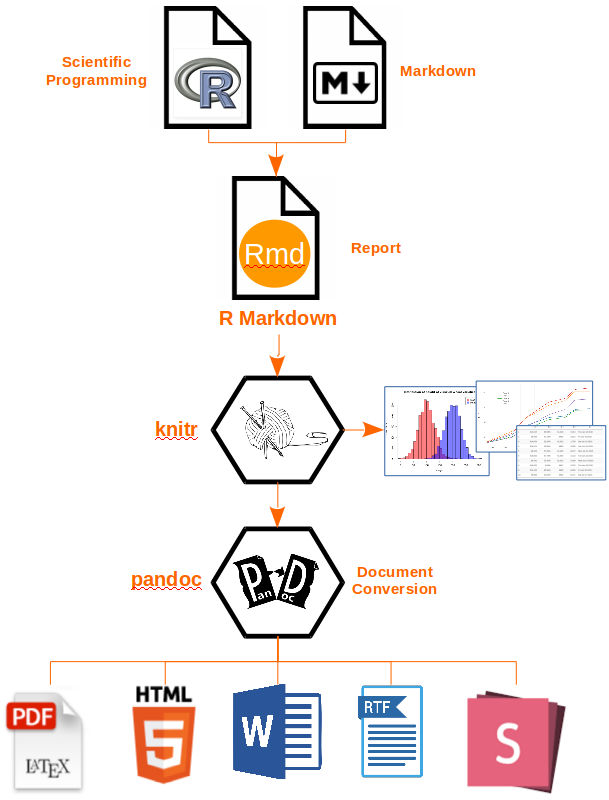
\includegraphics[width=3.76042in,height=\textheight]{rmarkdown_workflow.png}

\hypertarget{reproducibility}{%
\subsection{\texorpdfstring{\textbf{Reproducibility}}{Reproducibility}}\label{reproducibility}}

If there is already a published article and there is a new scientist who
wants to make an analyse using the same data from that article it will
only be reproducibility if the new result is the same as in the already
published article. There is benefits and disadvantages with
reproducibility and that is important to look into. Some scientists have
also tried to find some solution to the issues with mixing up
reproducibility, replicability and generalizability, because the
scientific environment have different opinions about what means what.

When the scientists agree on the definitions of the various terms, the R
notebook can be a good help further. As previously mentioned, the R
notebook is a good tool when it comes to organizing methods or results
so that it is reproducible. Using the R notebook will also make the
study more efficient and easier to share analyzes with other colleagues
or other scientists.

\hypertarget{benefits}{%
\subsubsection{Benefits}\label{benefits}}

As we have written about before, we use reproducibility to repeat a
research using the same data but with a separate twist.

Barbara R. Jasny et al.~writes in an article that new technology is
constantly emerging, and produces new data in different variants, which
increases the expectations for new knowledge. (Jasny et al. 2011). By
increasing the expectations of the data, we can also see an increase in
the expectations for the content.

Although a test is reproducible, the quality may not be as good.

\hypertarget{disadvantages}{%
\subsubsection{Disadvantages}\label{disadvantages}}

Steven N. Goodman et al.~are writing in their article that
reproducibility, replicability, reliability, robustness, and
generalizability are used interchangeably in, for example, scientific
environments. The terms seem to be a confusion in the literature and it
can make it difficult to rely on a scientific result For their part, it
is mostly for use in the biomedical field, but there is great faith that
this could also solve other scientific areas.@goodman\_what\_2016.

An example: Some groups believes reproducibility means repeating an
investigation in an article using the same data, and replicability means
doing it again, preferably with new data, but getting the same response.
While other groups believe the opposite.

There is also another minus with reproducibility and that is that the
result you have obtained can be built on by others who in turn can use
it to develop new ideas or other methods. It may lead to further errors
if the article was initially incorrect.

\href{https://www.jstor.org/stable/pdf/41352177.pdf?refreqid=excelsior\%3A4042fa72b0c4b5ce6ed25e118e92172a}{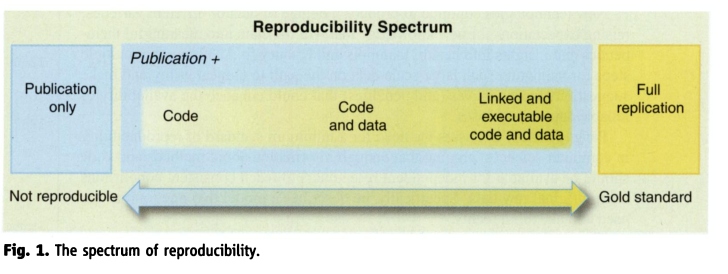
\includegraphics{Roger Peng.PNG}}

\hypertarget{solution}{%
\subsubsection{Solution}\label{solution}}

First of all, a solution could be that the scientific environment came
together to create and definition to each of the different concepts
reproducibility, replicability, reliability, robustness, and
generalizability. It would have made the concepts easier to use and
which in turn had given a common understanding of what was used at any
given time. Steven N. Goodman et al.~want to divide it into three
different elements: methods reproducibility, results reproducibility,
and inferential repro- ducibility. For their part, it is mostly for use
in the biomedical field, but there is great faith that this could also
solve other scientific areas Goodman, Fanelli, and Ioannidis (2016).

Bollen et al.~says that scientists should document all the information
in the procedures they use when collecting data - right down to the
level of detail. It will make it easier and more effective for
researchers who comes after using the same report and get the same
results as the original researchers. It will not only reproduce
reproducibility, but they will also be able to provide more information
Bollen et al. (2015).

\hypertarget{is-there-a-perfect-code}{%
\subsubsection{Is there a perfect code?}\label{is-there-a-perfect-code}}

Nick Barnes who works in the Climate Code Foundation writes in an
article from 2010, that researchers don't have to put so much emphasis
on coding in their work, because the benefit of sharing raw data can be
greater than writing a perfect code.

He further writes that if we share raw data that performs the job it is
supposed to, the intention with the data is in place. So why not share
it then.

He points out that in 2007 NASA released a software that wasn't
completely finished, but by releasing it before it was completely
finished, they received held along the way so that it became both better
and more user-friendly. Even if they got help, it didn't mean that NASA
had released a bad program or that the result after they released the
first version gave a slightly worse result. NASA took the change with
them and made the software even better.

In Conclusion, he writes that researchers must work together to create
space to release raw data, so that we can benefit from each other's help
to not always strive for perfectionism before we publish. But this is
not something researchers need to do alone they also need help from the
community around them (Barnes 2010)

\hypertarget{referances}{%
\subsubsection{\texorpdfstring{\emph{Referances}}{Referances}}\label{referances}}

\hypertarget{appendix}{%
\subsubsection{\texorpdfstring{\emph{Appendix}}{Appendix}}\label{appendix}}

Grolemund (n.d.)

rmarkdown\_workflow.png

Roger Peng.PNG

\begin{Shaded}
\begin{Highlighting}[]
\FunctionTok{sessionInfo}\NormalTok{()}
\end{Highlighting}
\end{Shaded}

\begin{verbatim}
## R version 4.1.1 (2021-08-10)
## Platform: x86_64-w64-mingw32/x64 (64-bit)
## Running under: Windows 10 x64 (build 19043)
## 
## Matrix products: default
## 
## locale:
## [1] LC_COLLATE=Norwegian Bokmål_Norway.1252 
## [2] LC_CTYPE=Norwegian Bokmål_Norway.1252   
## [3] LC_MONETARY=Norwegian Bokmål_Norway.1252
## [4] LC_NUMERIC=C                            
## [5] LC_TIME=Norwegian Bokmål_Norway.1252    
## 
## attached base packages:
## [1] stats     graphics  grDevices utils     datasets  methods   base     
## 
## loaded via a namespace (and not attached):
##  [1] compiler_4.1.1  magrittr_2.0.1  fastmap_1.1.0   tools_4.1.1    
##  [5] htmltools_0.5.2 yaml_2.2.1      stringi_1.7.4   rmarkdown_2.10 
##  [9] knitr_1.33      stringr_1.4.0   xfun_0.25       digest_0.6.27  
## [13] rlang_0.4.11    evaluate_0.14
\end{verbatim}

\hypertarget{refs}{}
\begin{CSLReferences}{1}{0}
\leavevmode\hypertarget{ref-barnes_publish_2010}{}%
Barnes, Nick. 2010. {``Publish {Your} {Computer} {Code}: {It} {Is}
{Good} {Enough}.''} \emph{Nature} 467 (7317): 753--53.
\url{https://doi.org/10.1038/467753a}.

\leavevmode\hypertarget{ref-bollen_social_2015}{}%
Bollen, Kenneth, John T. Cacioppo, Jon A. Krosnick, James L. Olds, and
Robert M. Kaplan. 2015. {``Social, {Behavioral}, and {Economic}
{Sciences} {Perspectives} on {Robust} and {Reliable} {Science}.''}
Report of the Subcommittee on Replicability in Science Advisory
Committee to the National Science Foundation Directorate for Social,
Behavioral, and Economic Sciences. NSF.

\leavevmode\hypertarget{ref-goodman_what_2016}{}%
Goodman, Steven N., Daniele Fanelli, and John P. A. Ioannidis. 2016.
{``What {Does} {Research} {Reproducibility} {Mean}?''} \emph{Science
Translational Medicine} 8 (341): 341ps12--12.
\url{https://doi.org/10.1126/scitranslmed.aaf5027}.

\leavevmode\hypertarget{ref-grolemund_r_nodate}{}%
Grolemund, Garrett, J. J. Allaire. n.d. \emph{R {Markdown}: {The}
{Definitive} {Guide}}. Accessed September 15, 2021.
\url{https://bookdown.org/yihui/rmarkdown/}.

\leavevmode\hypertarget{ref-jasny_again_2011}{}%
Jasny, Barbara R., Gilbert Chin, Lisa Chong, and Sacha Vignieri. 2011.
{``Again, and {Again}, and {Again}.''} \emph{Science} 334 (6060):
1225--25. \url{https://doi.org/10.1126/science.334.6060.1225}.

\leavevmode\hypertarget{ref-lander_r_2017}{}%
Lander, Jared P. 2017. \emph{R for {Everyone}: {Advanced} {Analytics}
and {Graphics}}. 2nd Edition. Boston: Addison-Wesley Professional.

\end{CSLReferences}

\end{document}
